



\documentclass[a4paper,12pt,spanish]{article}

\usepackage[utf8]{inputenc}


\usepackage{blindtext}
%\usepackage{microtype}
\usepackage{amsfonts, amsmath, amsthm, amssymb}
%\usepackage{fancyhdr}
%\usepackage{index}
%\usepackage{multicol}    

%\usepackage{booktabs}

\usepackage[T1]{fontenc}
\usepackage[utf8]{inputenc}
\usepackage{graphicx}
\usepackage[spanish,es-tabla]{babel}
\usepackage{url}
\usepackage{enumitem}

\usepackage[unicode=true, pdfusetitle,
bookmarks=true,bookmarksnumbered=false,bookmarksopen=false,
breaklinks=true,pdfborder={0 0 1},backref=false,colorlinks=false]
{hyperref}

\usepackage{listings}
\usepackage{longtable}


\usepackage{siunitx} %para el sistema internacional
\usepackage[export]{adjustbox}
\usepackage{booktabs} 
\usepackage{subcaption}

\usepackage{float}


\newcommand{\address}[1]{
	\par {\raggedright #1
		\vspace{1.4em}
		\noindent\par}
}

\usepackage[table,xcdraw]{xcolor}


\pagenumbering{gobble}
\include{noNumberPage}
\pagenumbering{arabic}
\setcounter{page}{11}

%tutorial de tablas latex: https://manualdelatex.com/tutoriales/tablas

\usepackage{multirow}

% \usepackage[table,xcdraw]{xcolor}


%Inicio del documento (hasta que se cierre con \end{document}
\begin{document}
	
	
	\title{ Absorción de Partículas Beta}
	
	%\author{Adrián Rivero Fernández}
	\date{}
	
	\maketitle
	
	
	\section{Objetivos de la práctica}
	
	\vspace{\baselineskip}
	
	1. Determinar la curva del alcance en función del espesor de absorbente de aluminio para una fuente de $\text{Sr}^{90}$\\
	
	2. Determinar el alcance a partir de la gráfica.\\
	
	3. Determinar la energía máxima de las partículas $\beta$.\\
	
	4. Comparar los resultados experimentales con los obtenidos a partir de la fórmula de Feather.\\
	
	
	
	
	
	\section{Curva de alcance-espesor}
	
	Para un tiempo de acumulación de 90 segundos, medimos la radiación del $\text{Sr}^{90}$ para distintos espesores de Aluminio, que determinamos añadiendo placas apiladas entre el emisor y el detector. Obtenemos la Tabla 1. 
	
	
	
	\begin{table}[H]
		\centering
		\begin{tabular}{|c|c|c|}
			\hline
			Espesor (mm) & Espesor ($\si{g/cm^2}$) & Cuentas \\ \hline\hline
			0            & 0                     & 20352   \\ \hline
			0,4          & 0,11                  & 13581   \\ \hline
			0,8          & 0,22                  & 8564    \\ \hline
			1,2          & 0,33                  & 5225    \\ \hline
			1,6          & 0,44                  & 2839    \\ \hline
			2            & 0,55                  & 1480    \\ \hline
			2,4          & 0,66                  & 727     \\ \hline
			2,8          & 0,77                  & 332     \\ \hline
			3,2          & 0,88                  & 145     \\ \hline
			3,6          & 0,99                  & 94      \\ \hline
			4            & 1,1                   & 62      \\ \hline
			4,4          & 1,21                  & 65      \\ \hline
			5,6          & 1,54                  & 60      \\ \hline
		\end{tabular}
		\caption{Medida de radiación para 90s según el espesor}
	\end{table}
	
	
	Representando estos datos, obtenemos la gráfica de radiación según el espesor, que representamos en escala semilogarítmica.
	
\begin{figure}[H]
	\centering
	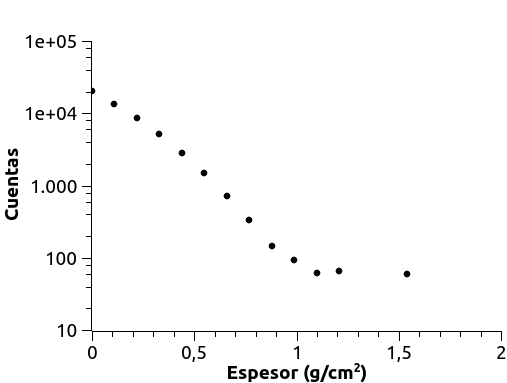
\includegraphics[width=0.7\linewidth]{imagenes/grafica_log_1-2}
	\caption{Partículas $\beta$ en función del espesor}
	\label{fig:graficalog1-2}
\end{figure}
	
	
	
	Podemos el alcance en 1,1 $\si{g/cm^2}$, ya que se estabiliza en ese punto. \\
	
	
	Para esta parte que se comporta de forma exponencial, podemos obtener la expresión de la curva representando el logaritmo de la radiación frente al espesor y ajustando la recta:
	
	\begin{figure}[H]
		\centering
		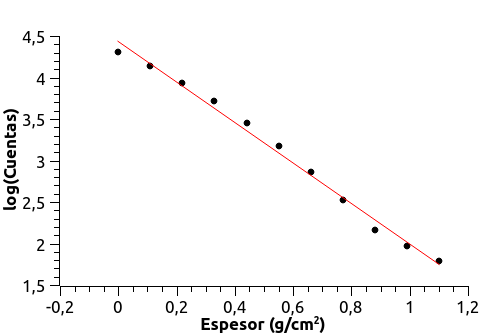
\includegraphics[width=0.7\linewidth]{imagenes/grafica_log_10}
		\caption{Ajuste de la región exponencial}
		\label{fig:graficalog10}
	\end{figure}
	
	
	donde la recta de ajuste, siendo $N$ el número de cuentas y $X$ el espesor, es:
	
	\[\log N = -2,44 X + 4,43\]
	\[N = 10^{(-2,44 X + 4,43)}\]
	
	%B=4.43501472120952
	%A=-2.43964842791722
	
	%A*x+B
	
	Interpolando con esta expresión para el valor del fondo de radiación (medido para prácticas anteriores, $F = 54$), podemos estimar el punto en que la curva quedará horizontal:
	
	\[ 54 = 10^{(-2,44 X + 4,43)} \longrightarrow X = 1,1 \si{g/cm^2}
	\]
	
	\section{Energía máxima}
	
	
	A partir de la Tabla II del guión, representamos la energía máxima de partículas $\beta$ según su alcance.
		
	\begin{figure}[H]
		\centering
		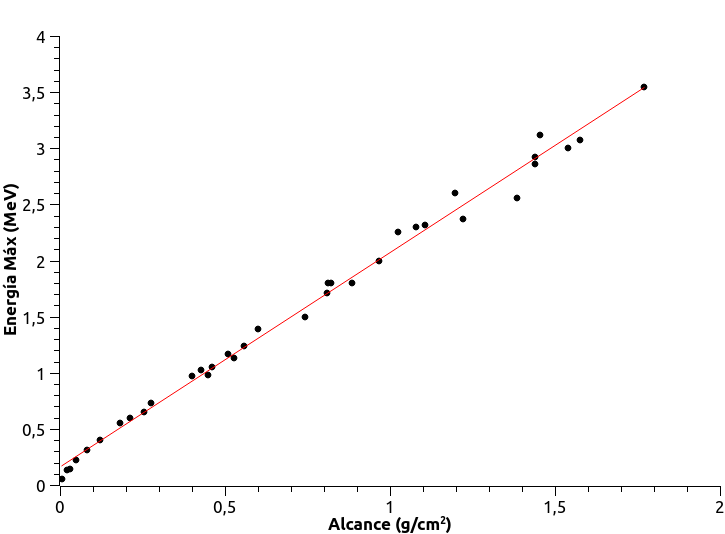
\includegraphics[width=0.7\linewidth]{imagenes/nueva_copiar}
		\caption{Alcance de las partículas $\beta$ en función de la energía máxima}
		\label{fig:graficaenergiabuena}
	\end{figure}
	%B=0.16194579749683
	%A=1.90916819778655
	
	%A*x+B
	
	La recta de ajuste de la Figura 3 es
	\[ T = 1,91 X + 0,17
	\]
	
	Interpolando para $X = 1,1$ podemos establecer la energía máxima:
	\[ T_{1,1} = 2,27 \si{MeV}
	\]
	
	
	La energía máxima para el $\text{Sr}^{90}$ que aparece en los esquemas de desintegración es de 2,28 MeV, aplicando las fórmulas de \textit{Feather}:
	
	\[T= 2,28 \si{MeV}\]
	\[T = 1,845\times R + 0,245\]
	\[R = \frac{T - 0,245}{1,845} \longrightarrow R = 1,1 (\si{g/cm^2})\]
	
	Podemos ver que el tanto el alcance medido y el calculado como las energías máximas son iguales.
	
	

	
	
	
	
	
\end{document}